\section{The Direction Is Reproducible Only Because Prompts Have Identities}
\label{sec:stability}

\Cref{tab:stability} reports the split-half cosine at the two levels. The contrast between the
columns is the central empirical fact of this paper.

\begin{table}[t]
\centering
\scriptsize
\setlength{\tabcolsep}{4pt}
\begin{tabular}{lccccc}
\toprule
Model & Pooled & Within & 95\% CI & $>0.5$ & $p$ \\
\midrule
pythia-410m  & $+0.999$ & $-0.037$ & $[-0.222, 0.149]$ & 12/40 & 0.701 \\
pythia-1b    & $+0.999$ & $-0.119$ & $[-0.327, 0.089]$ & 13/40 & 0.268 \\
pythia-2.8b  & $+0.532$ & $+0.035$ & $[-0.029, 0.100]$ & 1/40  & 0.287 \\
SmolLM2      & $-0.635$ & $-0.021$ & $[-0.111, 0.069]$ & 3/40  & 0.651 \\
Qwen-1.5B    & $-0.482$ & $+0.063$ & $[-0.014, 0.141]$ & 1/40  & 0.119 \\
Qwen-7B      & $-0.758$ & $-0.029$ & $[-0.115, 0.056]$ & 1/40  & 0.507 \\
OLMo-2-7B    & $-0.534$ & $-0.068$ & $[-0.149, 0.014]$ & 1/40  & 0.111 \\
\bottomrule
\end{tabular}
\caption{Split-half stability of the contrast direction. \emph{Pooled}: cosine between directions
fitted on two random halves of the full sample set, with prompts mixed. \emph{Within}: mean cosine
over prompts between directions fitted on two disjoint halves of a single prompt's own 32 responses;
the interval is a $95\%$ $t$-interval over the 40 prompts, $p$ tests the mean against zero, and
$>0.5$ counts prompts above that cosine. The pooled fit is essentially perfect for the base models
and strongly negative for the instruction-tuned ones, yet the within-prompt fit is indistinguishable
from zero in every model.}
\label{tab:stability}
\end{table}

\paragraph{The pooled fit is stable, and negative.}
The two base models with the largest effective sample agreement, pythia-410m and pythia-1b, give a
pooled cosine of $+0.999$: two independent halves yield the same vector to three decimals. This is
what makes the recipe look sound, and what a practitioner would cite as evidence that the estimator
works. For the instruction-tuned models the pooled cosine is instead large and negative, between
$-0.48$ and $-0.76$, corresponding under $\cos = (\lVert \Delta \rVert^2 - \lVert \varepsilon
\rVert^2)/(\lVert \Delta \rVert^2 + \lVert \varepsilon \rVert^2)$ to a signal-to-noise ratio
below one. Either way the statistic looks informative, once positive and once negative, and in
neither case does it license the inference that a diversity axis has been found.

\paragraph{The within-prompt fit is not stable at all.}
When the two halves are drawn from the same prompt, the agreement collapses. Across all seven models
the mean within-prompt cosine lies between $-0.119$ and $+0.063$, no model differs significantly
from zero (all $p > 0.11$), and in five of seven models at most three of the forty prompts exceed a
cosine of $0.5$. The exceptions are the base models pythia-410m and pythia-1b, at twelve and
thirteen prompts out of forty; even there the mean stays negative, so the distribution is bimodal
around zero rather than concentrated at a usable value. A direction that predicts its own other half
in one prompt in three cannot support an intervention.

\paragraph{The gap is the finding.}
For pythia-410m the same estimator, the same quantiles, and the same activations yield $+0.999$ at
the pooled level and $-0.037$ at the within-prompt level. The only difference is whether the two
halves may contain responses to different prompts. If the direction measured dispersion, restricting
the comparison to a single prompt would remove between-prompt variance and leave the dispersion
signal intact or clearer; instead it removes the entire reproducible component. What the pooled
estimator recovers is therefore a direction that separates prompts from one another, which is
stable because each prompt has a characteristic mean activation, and which has nothing to say about
which of that prompt's responses are varied.

\paragraph{Consequence for the pooled vector.}
Write $v_{\text{pool}} \approx \frac{1}{P}\sum_p s_p v_p$ with $s_p \in \{\pm 1\}$ the sign
induced by pooling. If the $v_p$ were aligned the sum would grow linearly in $P$ and have a
meaningful direction; if they are orthogonal the norm grows only as $\sqrt{P}$ and the direction is
set by whichever prompts contribute largest. A direct check confirms the latter: the mean pairwise
cosine between per-prompt fits is $+0.010$ to $+0.018$ for Qwen2.5-7B and OLMo-2-7B and never exceeds
$+0.16$ for any model. The $+0.999$ agreement therefore reflects the reproducible identity component
of each prompt, not a coherent direction in the sum.

\begin{figure}[t]
\centering
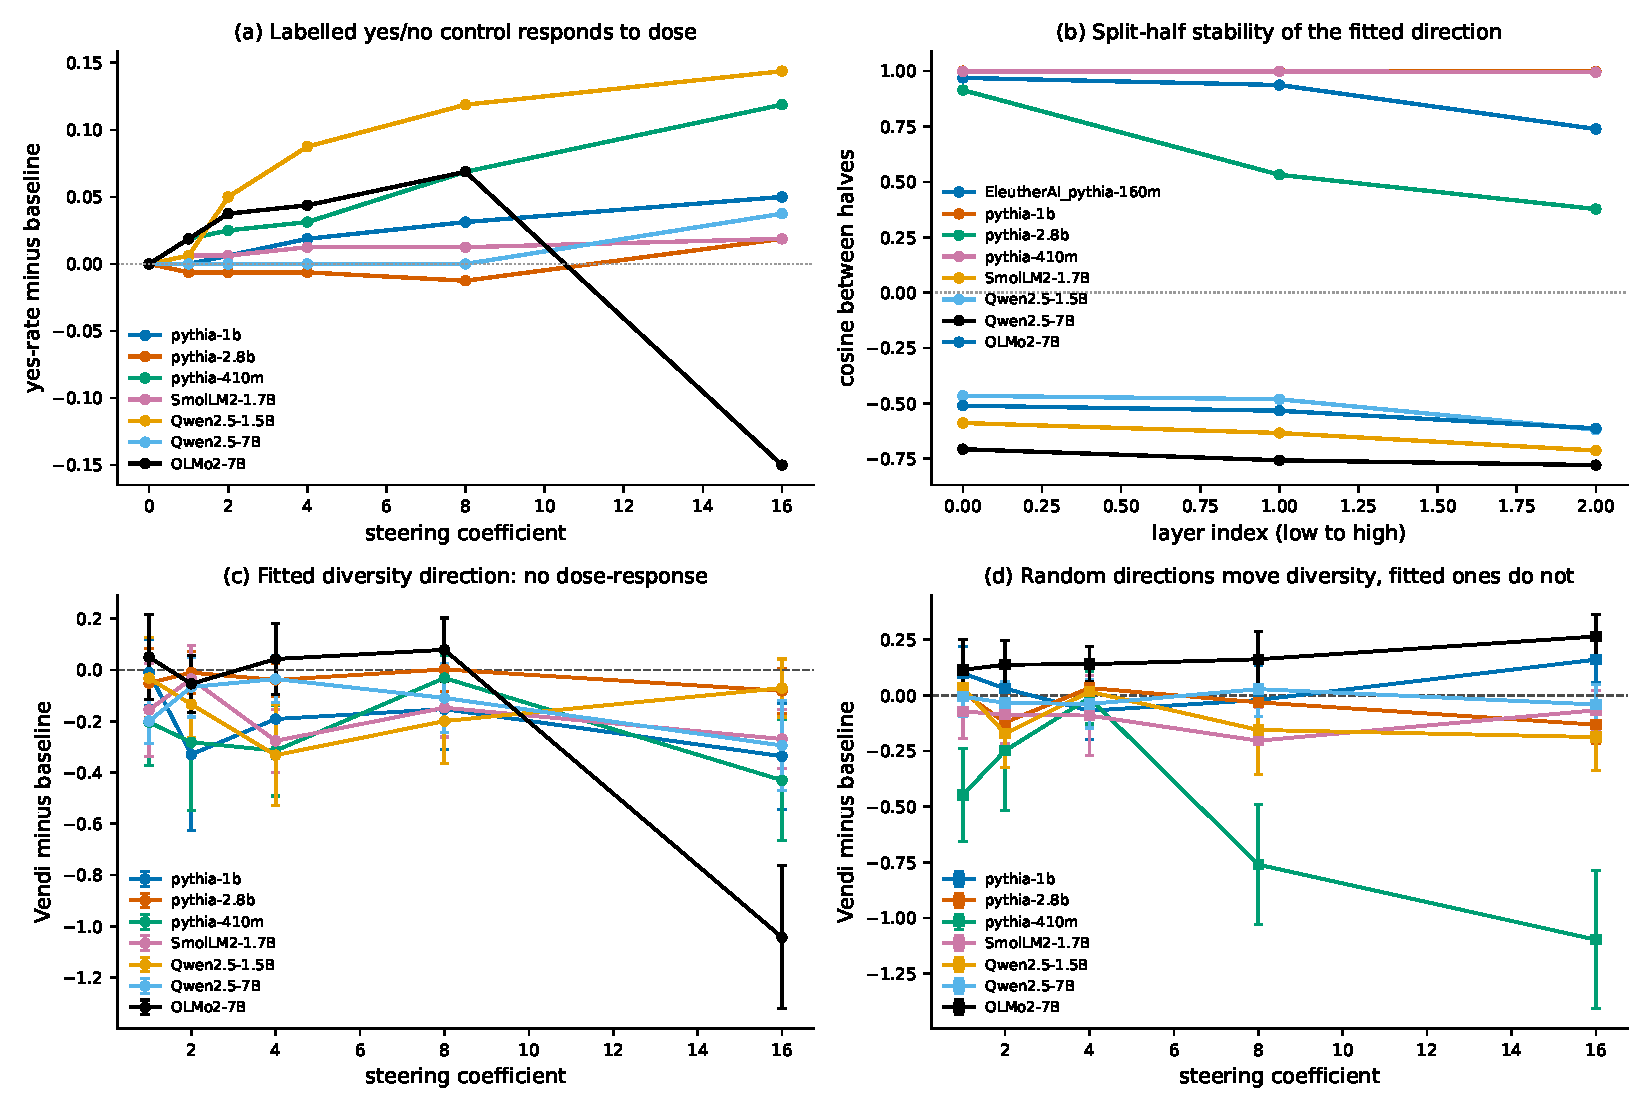
\includegraphics[width=0.94\linewidth]{figures/confirm.pdf}
\caption{Confirmatory evidence. (a) A labelled yes/no direction produces a monotone dose-response in
the same pipeline, establishing that the interventions do reach the model. (b) Pooled split-half
stability, which separates base from instruction-tuned models but, as \Cref{tab:stability} shows,
does not survive the within-prompt restriction. (c) The fitted diversity direction produces no
dose-response in any model. (d) Random directions of the same norm move \vendi{} more than the
fitted direction, and in the direction of degeneration rather than control.}
\label{fig:confirm}
\end{figure}
